\section{Análisis empírico}

\subsection{Performance para distribuciones uniforme}
A continuación mostraremos cómo se comportaron los distintos estimadores en cuanto al error medio obtenido ante la variación del parámetro $p$ de entrada del estimador. Para cada $p$, fueron realizadas $N$ consultas por igualdad y $N$ consultas por mayor.  


\begin{figure}[h!]  
  \centering
  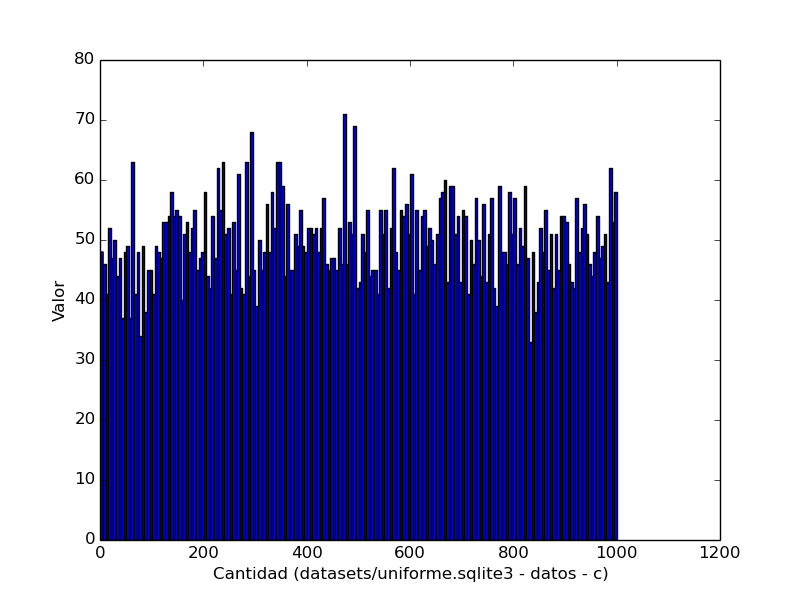
\includegraphics[width=0.45\textwidth]{../source/datasets/img/uniforme}
  \caption{Distribución utilizada}
 \end{figure}
 
\begin{figure}[h!]  
  \centering
  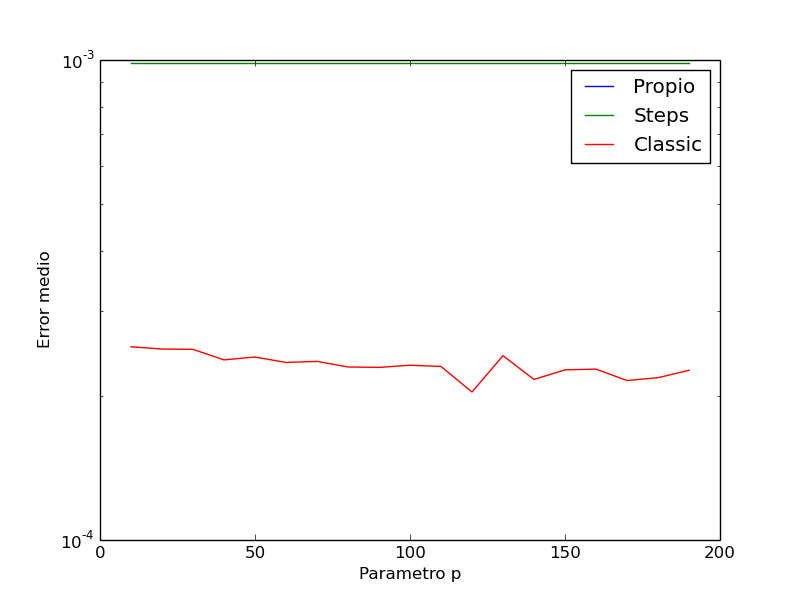
\includegraphics[width=0.45\textwidth]{../source/datasets/img/uniformeEqual}
  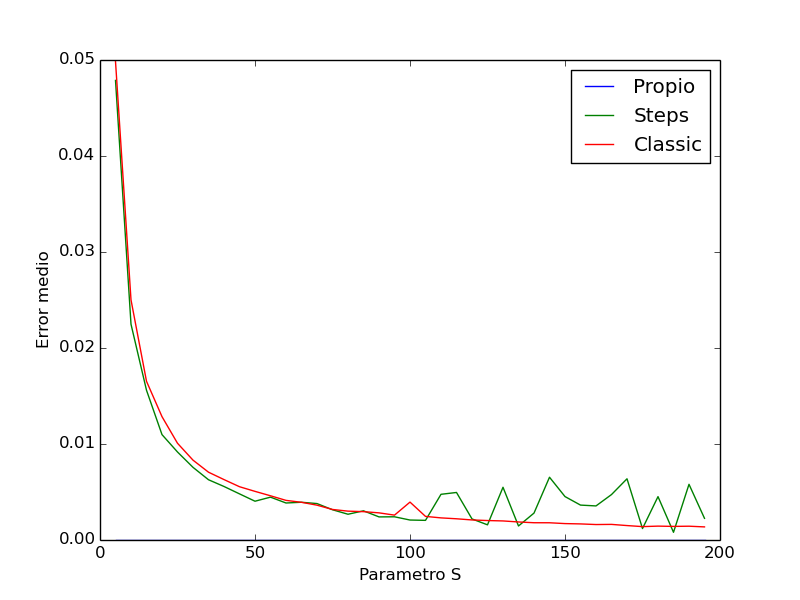
\includegraphics[width=0.45\textwidth]{../source/datasets/img/uniformeGreater}
  \caption{Gráficos para distribución uniforme, con consultas por igualdad y por mayor respectivamente.}
 \end{figure}
 
 \subsubsection*{Análisis}
Estos datos confirman gran parte del análisis teórico que hicimos en la sección anterior. En primer lugar podemos ver cómo, en el caso de la estimación por igualdad, la elección del parámetro del estimador no modifica de manera alguna la performance. Además, en ese caso la performance de ambos estimadores es muy buena (entre 0.0002 y 0.001), como también habíamos predicho. En el caso de la estimación por mayor confirmamos que, en ambos estimadores, a diferencia de la estimación por igualdad, la elección del parámetro cambia drásticamente la performance obtenida, mejorandola al elevar el valor del parámetro. Un resultado que no estaba contemplado en el análisis teórico que a partir de cierto valor del parámetro la performance del estimador Distribution Steps cambia erráticamente, creemos que esto se debe a que llega cierto punto en el que, al tener muchos steps, empieza a haber valores que aparecen en más de un límite. Y en esa situación el algoritmo, si bien intenta minimizar el error en el caso promedio, pierde precisión al no poder ubicar unívocamente en qué bucket cae el valor de la consulta.
 
 \subsection{Performance para distribuciones normal}
A continuación mostraremos cómo se comportaron los distintos estimadores en cuanto al error medio obtenido ante la variación del parámetro $p$ de entrada del estimador. Para cada $p$, fueron realizadas $N$ consultas por igualdad y $N$ consultas por mayor.  


\begin{figure}[h!]  
  \centering
  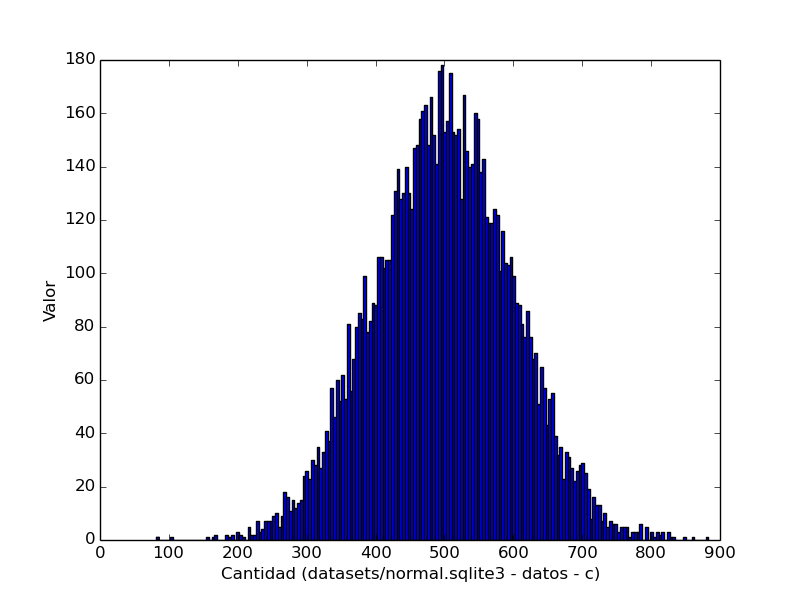
\includegraphics[width=0.45\textwidth]{../source/datasets/img/normal}
  \caption{Distribución utilizada}
 \end{figure}

\begin{figure}[h!]
  \centering
  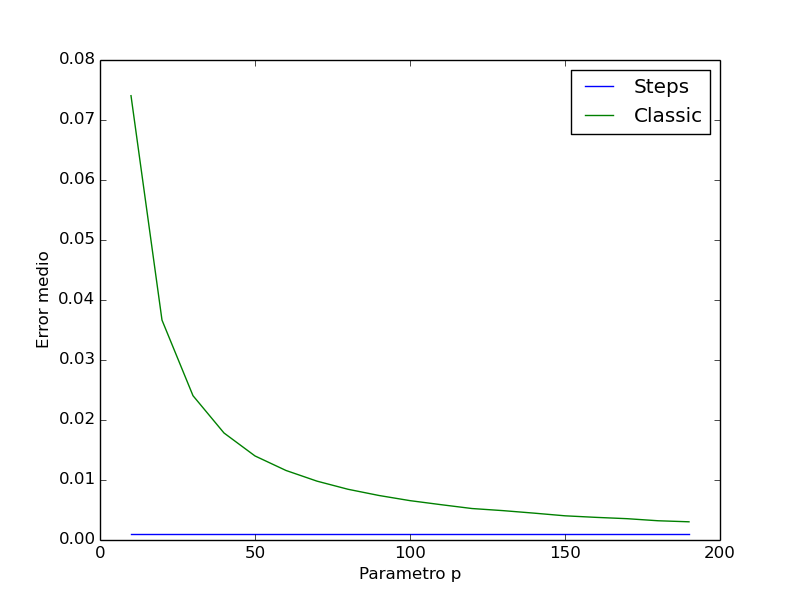
\includegraphics[width=0.45\textwidth]{../source/datasets/img/normalEqual}
  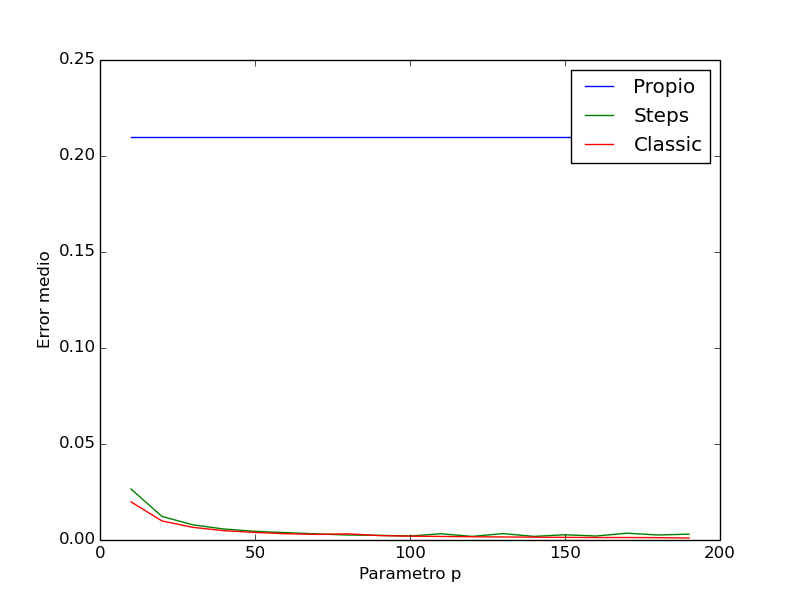
\includegraphics[width=0.45\textwidth]{../source/datasets/img/normalGreater}
  \caption{Gráficos para distribución normal, con consultas por igualdad y por mayor respectivamente.}
 \end{figure}

 \subsubsection*{Análisis}
Gran parte del análisis es similar al caso uniforme con la excepción de que, como dijimos en el análisis teórico, el estimador clásico debería aumentar la performance al aumentar el parámetro. Esta mejora se aprecia únicamente en los primeros valores del experimento ya que llega rápidamente a una cantidad de buckets que le permite armar un histograma que caracteriza con precisión la distribución de este dataset. En este caso puede verse que el valor se encuentra alrededor de 10 pero en otros datasets este valor podría cambiar en incluso necesitarse muchos más buckets para llegar al máximo nivel de performance.

\subsection{Performance para diferentes distribuciones}
En esta sección calculamos la performance de los estimadores en datasets de diferentes distribuciones provistas por la cátedra y análizamos, en cada caso, mediante un test de hipótesis, si alguno de los estimadores es significativamente mejor o si, en términos estadísticos, no existe una diferencia importante de performance. 
El test utilizado es el \textit{Student’s T-Test Apareado} y para realizarlo necesitamos tener dos conjuntos de datos emparentados que representen la información que queremos comparar. En nuestro caso, para comparar el estimador $A$ con el estimador $B$ en cierto dataset, calculamos por un lado la performance de $A$ para estimar valores individuales del dataset y, por otro lado, la performance de $B$ para estimar esos mismos valores. Esto nos da dos listas de datos que están emparentadas por los valores que se estan estimando. Los valores a estimar cubren todo el rango de valores del dataset en intervalos de 10 unidades. Era necesario calcular la performance individual para diferentes valores del dataset y no simplemente tomar la performance como el promedio de todos esos valores ya que el valor promedio no es suficiente información para llevar adelante un test de hipótesis de estas características.

Presentamos a continuación los gráficos de los datasets utilizados:

\begin{figure}[h!]
  \centering
  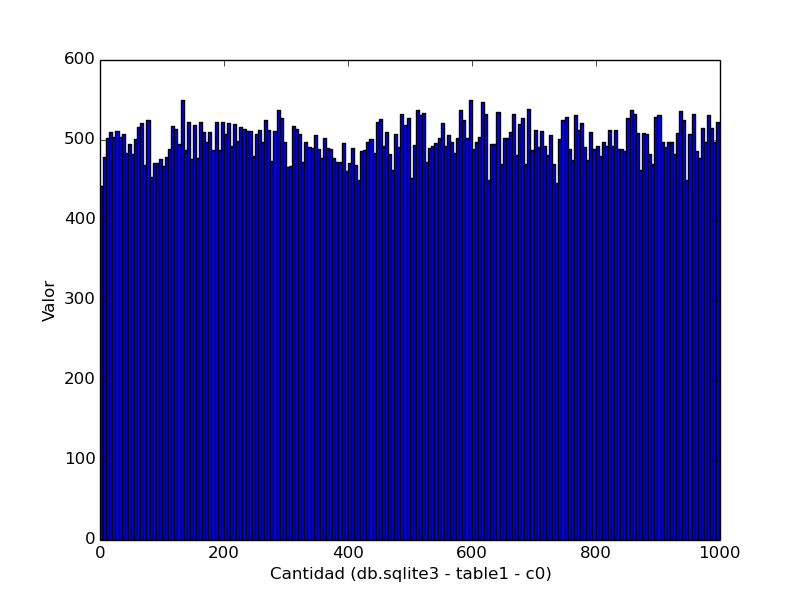
\includegraphics[width=0.45\textwidth]{./../source/datasets/img/c0}
  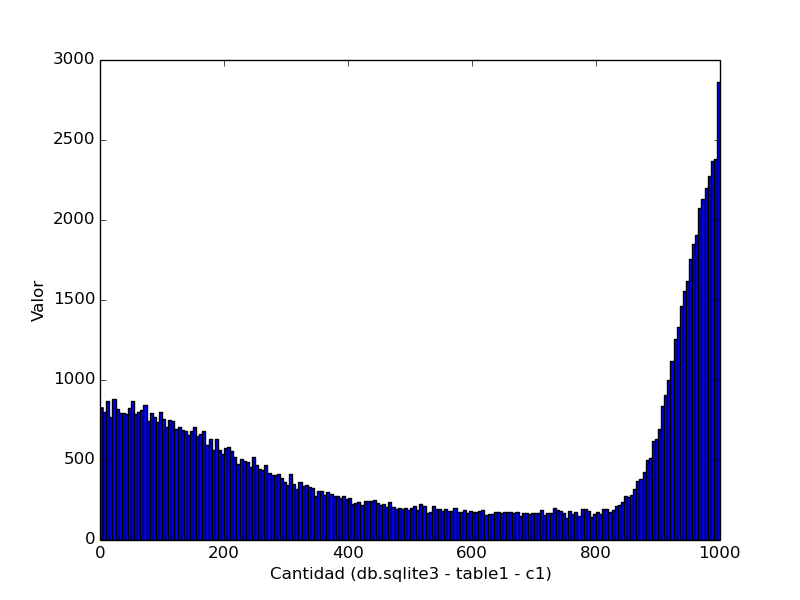
\includegraphics[width=0.45\textwidth]{./../source/datasets/img/c1}
  \caption{Gráficos de los datasets de las columnas c0 y c1}
 \end{figure}
 
 
\begin{figure}[h!]
  \centering
  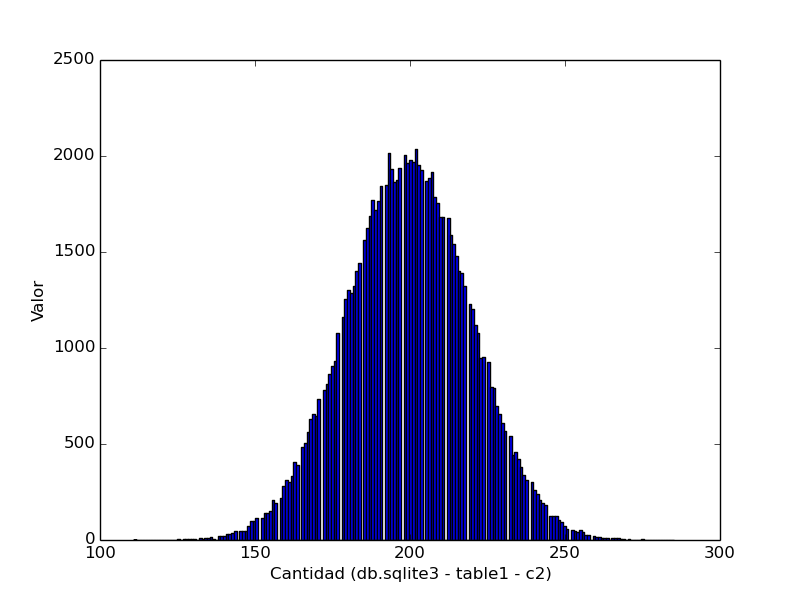
\includegraphics[width=0.45\textwidth]{./../source/datasets/img/c2}
  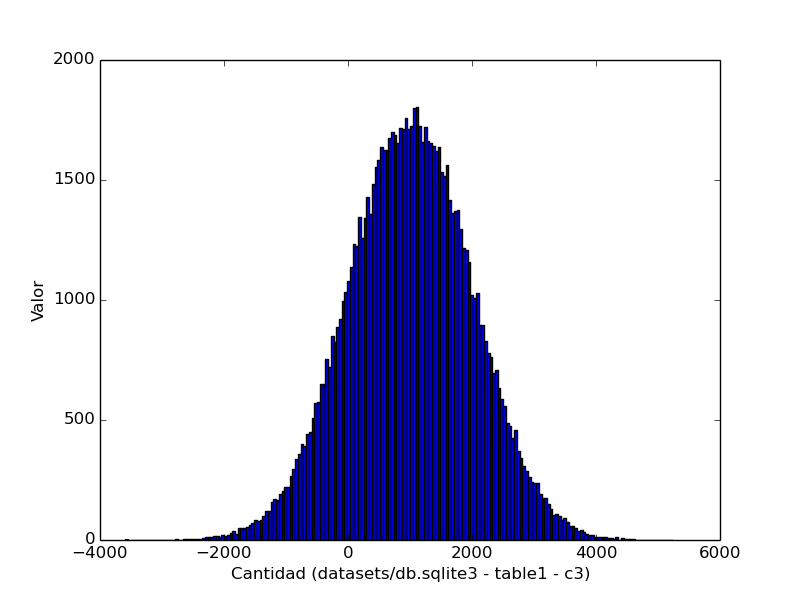
\includegraphics[width=0.45\textwidth]{./../source/datasets/img/c3}
  \caption{Gráficos de los datasets de las columnas c2 y c3}
 \end{figure}
 
\begin{figure}[h!]
  \centering
  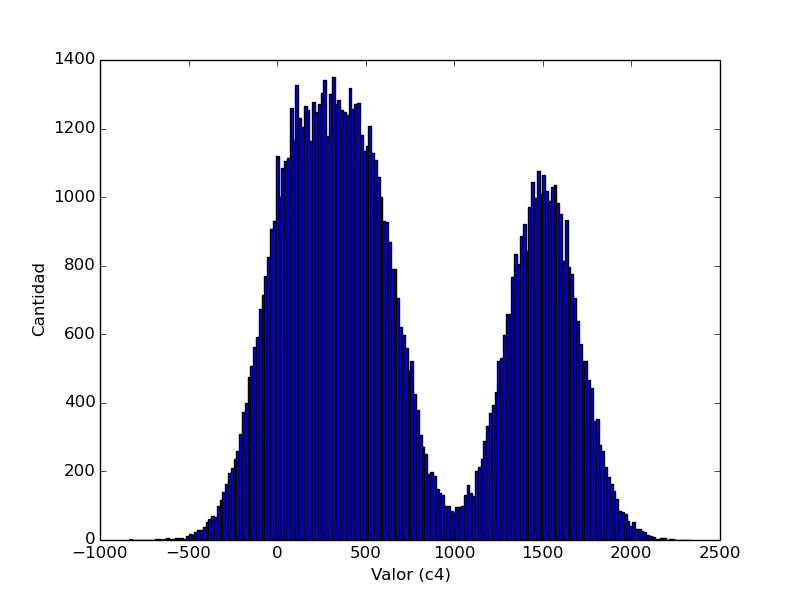
\includegraphics[width=0.45\textwidth]{./../source/datasets/img/c4}
  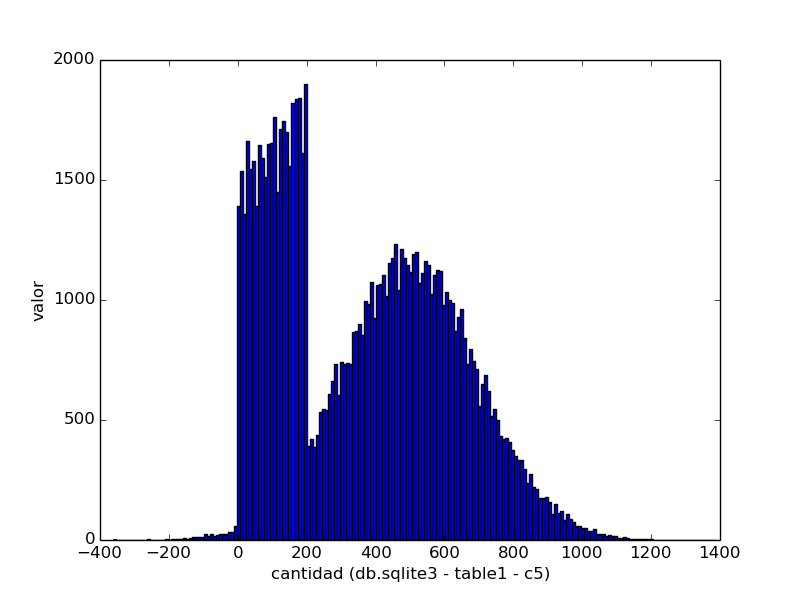
\includegraphics[width=0.45\textwidth]{./../source/datasets/img/c5}
  \caption{Gráficos de los datasets de las columnas c4 y c5}
 \end{figure}
 
 
\begin{figure}[h!]
  \centering
  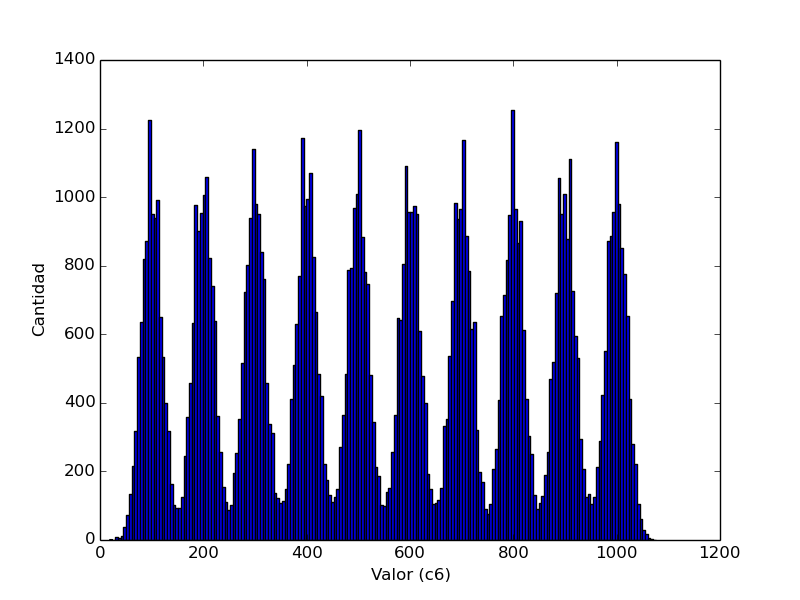
\includegraphics[width=0.45\textwidth]{./../source/datasets/img/c6}
  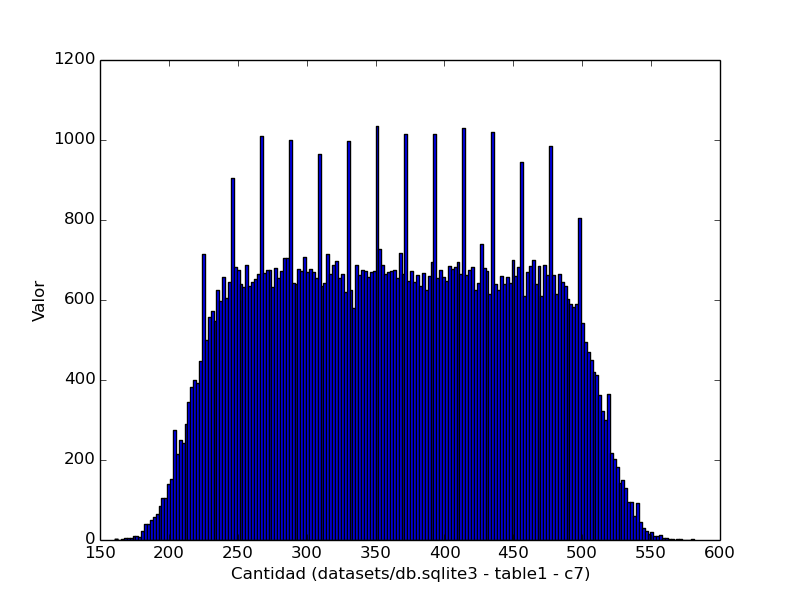
\includegraphics[width=0.45\textwidth]{./../source/datasets/img/c7}
  \caption{Gráficos de los datasets de las columnas c6 y c7}
 \end{figure}
 
 
\begin{figure}[h!]
  \centering
  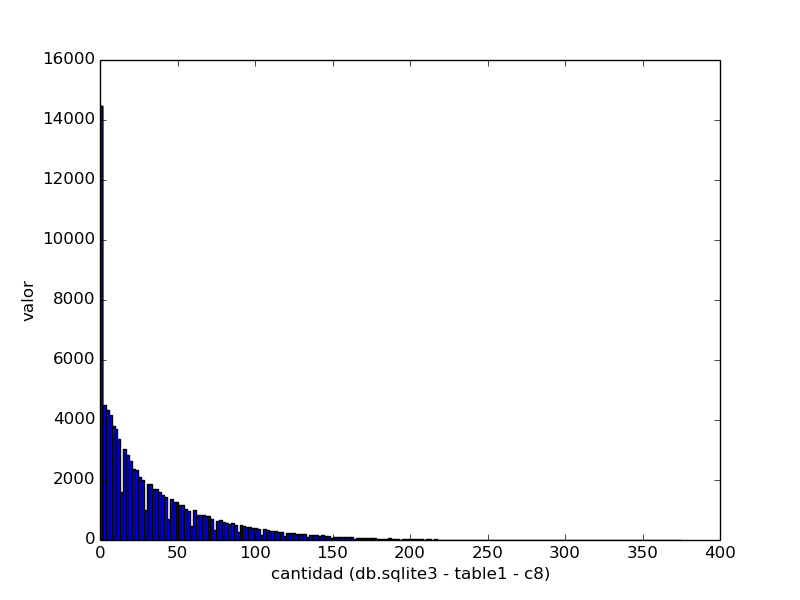
\includegraphics[width=0.45\textwidth]{./../source/datasets/img/c8}
  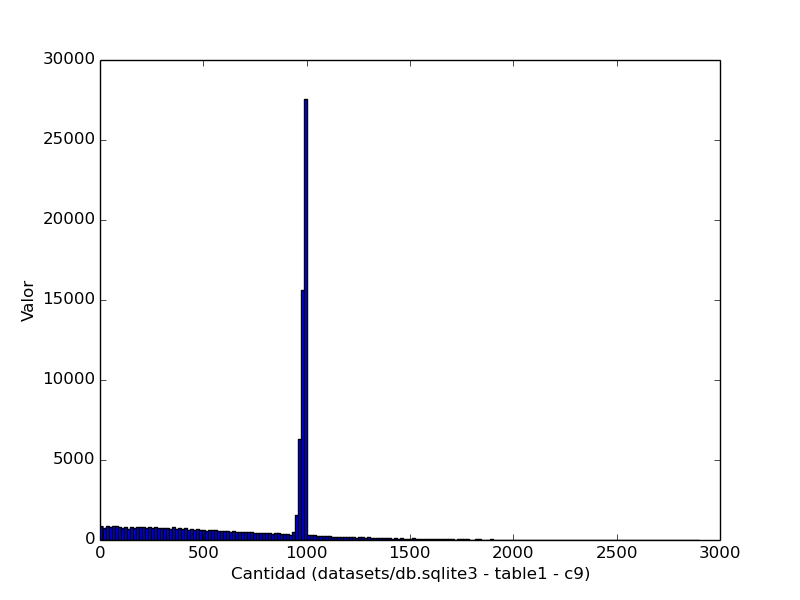
\includegraphics[width=0.45\textwidth]{./../source/datasets/img/c9}
  \caption{Gráficos de los datasets de las columnas c8 y c9}
 \end{figure}
 
 

\newpage

\begin{table}[h!t]
\centering % centering table
\begin{tabular}{c rrrrrrr} % creating eight columns
\hline\hline %inserting double-line
\ &\multicolumn{2}{c}{Propio}& \multicolumn{2}{c}{Classic}& \multicolumn{2}{c}{Steps} \\ [0.5ex] 
\hline % inserts single-line
 & E & G & E & G & E & G &  \\  
\hline
Propio &X  &X  &0-9 &0-9 &0-9 &0-9 \\ % Entering row contents
\hline
Classic &8  &-  &X &X &1-9 &6 \\
\hline
Steps &-  &- &- &0,3-5 &X &X  \\[1ex] % [1ex] adds vertical space
\hline % inserts single-line
\end{tabular}
\caption{Comparación entre estimadores de cual es más significativo, en qué tipo consulta y en qué columnas. } %title of the table
\label{tab:hresult}
\end{table}

\subsubsection*{Análisis}
Como se puede apreciar en \ref{tab:hresult} podemos notar como el estimador creado por nosotros, se queda con todas las ``competencias'' entre los estimadores. Esto es debido a que nuestro estimador es perfecto. Es decir, siempre devolverá la probabilidad exacta del cumplimiento de la consulta (o de una parte de ella). Igualmente vale remarcar que el estimador ``Classic'' logró empatar (no marcar una diferencia significaente según el \textit{Student’s T-Test Apareado}) con el estimador perfecto, lo cual significa que anduvo muy bien en ese caso.
